\documentclass[10pt]{article}
\usepackage{graphicx}
\usepackage{fullpage}
\usepackage[hidelinks]{hyperref}
\usepackage{amsfonts}
\usepackage{amsmath}
\usepackage{amssymb}
\usepackage{amsthm}
\usepackage{bbm}
\usepackage{natbib}
\usepackage{clrscode3e}

% Basic mathematical notation
\newcommand{\R}{\mathbb{R}}
\newcommand{\E}{\mathbb{E}}
\newcommand{\expct}[1]{\E\left[#1\right]}
\renewcommand{\P}{\mathbb{P}}
\newcommand{\one}{\mathbb{I}}
\newcommand{\mat}[1]{\mathbf{#1}}
%\newcommand{\dim}{\operatorname{dim}}
\newcommand{\rank}{\operatorname{rank}}
\newcommand{\diag}{\operatorname{diag}}
\newcommand{\vecm}{\operatorname{vec}}
\newcommand{\dist}{\mathsf{dist}}
\newcommand{\norm}[1]{\|#1\|}
\newcommand{\sval}{\mathfrak{s}}

% Names of norms and vector spaces
\newcommand{\ltwo}{\ell^2}
\newcommand{\lone}{\ell^1}
\newcommand{\lp}{\ell^p}
\newcommand{\lpq}{\ell^q}
\newcommand{\ltworat}{\ell^2_{\cR}}
\newcommand{\lonerat}{\ell^1_{\cR}}
\newcommand{\lprat}{\ell^p_{\cR}}
\newcommand{\inner}[2]{\langle #1, #2 \rangle}

% Notation for MPD and POMDP
\newcommand{\mdp}{\langle S, A, T, r, d_0\rangle}
\newcommand{\pomdp}{\langle S, A, T, r, \Omega, O, \bzero \rangle}
% Notation for weighted automata
\newcommand{\sstar}{\Sigma^\star}
\newcommand{\cF}{\mathcal{F}}
\newcommand{\cR}{\mathcal{R}}
\newcommand{\A}{\mat{A}}
\newcommand{\B}{\mat{B}}
\newcommand{\ahist}{\boldsymbol{\alpha}_h}
\newcommand{\bhist}{\boldsymbol{\beta}_h}
\newcommand{\azero}{\boldsymbol{\alpha}_0}
\newcommand{\tazero}{\tilde{\boldsymbol{\alpha}}_0}
\newcommand{\hazero}{\hat{\boldsymbol{\alpha}}_0}
\newcommand{\ainf}{\boldsymbol{\alpha}_{\infty}}
\newcommand{\hainf}{\hat{\boldsymbol{\alpha}}_{\infty}}
\newcommand{\tainf}{\tilde{\boldsymbol{\alpha}}_{\infty}}
\newcommand{\bzero}{\boldsymbol{\beta}_0}
\newcommand{\binf}{\boldsymbol{\beta}_{\infty}}
\newcommand{\wa}{\langle \azero, \ainf, \{\A_\sigma\} \rangle}
\newcommand{\wA}{\langle \azero, \{\A_\sigma\} \rangle}
\newcommand{\waS}{\langle \azero, \ainf, \{\A_\sigma\}_{\sigma \in \Sigma} \rangle}
\newcommand{\wbS}{\langle \bzero, \binf, \{\B_\sigma\}_{\sigma \in \Sigma} \rangle}
\newcommand{\waQ}{\langle \mQ^\top \azero, \mQ^{-1} \ainf, \{\mQ^{-1} \A_\sigma
\mQ\} \rangle}
\newcommand{\hwa}{\langle \hazero, \hainf, \{\hat{\A}_\sigma\} \rangle}
\newcommand{\twa}{\langle \tazero, \tainf, \{\tilde{\A}_\sigma\} \rangle}
\newcommand{\wb}{\langle \bzero, \binf, \{\B_\sigma\} \rangle}
\newcommand{\waV}{\langle \azero, \phi, \{\tau_\sigma\} \rangle}
\newcommand{\wasigma}{\langle \azero, \ainf, \{\A_\sigma\}_{\sigma \in \Sigma} \rangle}
\newcommand{\alamb}{\boldsymbol{\alpha}_{\lambda}}
\newcommand{\ainfa}{\boldsymbol{\alpha}_{a}}
\newcommand{\wapS}{\langle \alamb, \{\ainfa\}_{a \in A}, \{\A_\sigma\}_{\sigma \in \Sigma} \rangle}
\newcommand{\wap}{\langle \alamb, \{\ainfa\}, \{\A_\sigma\} \rangle}
\newcommand{\wAp}{\langle \alamb, \{\A_\sigma\} \rangle}

% Sets with name
\newcommand{\Ps}{\mathcal{P}}
\newcommand{\Ss}{\mathcal{S}}
\newcommand{\cD}{\mathcal{D}}
\newcommand{\cA}{\mathcal{A}}
\newcommand{\cB}{\mathcal{B}}

% Special norms
\newcommand{\normop}[1]{\|#1\|_{\mathrm{op}}}
\newcommand{\normhk}[1]{\|#1\|_{\mathrm{hk}}}

% (Blocks of) Hankel matrices
\renewcommand{\H}{\mat{H}}
\newcommand{\hr}{\mat{h}_{\lambda,\Ss}}
\newcommand{\hc}{\mat{h}_{\Ps,\lambda}}

% Named matrices and vectors
\renewcommand{\v}{\mat{v}}
\newcommand{\mM}{\mat{M}}
\newcommand{\mP}{\mat{P}}
\newcommand{\mS}{\mat{S}}
\newcommand{\mG}{\mat{G}}
\newcommand{\mU}{\mat{U}}
\newcommand{\mV}{\mat{V}}
\newcommand{\mD}{\mat{D}}
\newcommand{\mQ}{\mat{Q}}
\newcommand{\mI}{\mat{I}}
\newcommand{\mT}{\mat{T}}
\renewcommand{\mp}{\mat{p}}
\newcommand{\me}{\mat{e}}

% Environments for mathematical statements
\newtheorem{theorem}{Theorem}
\newtheorem{proposition}[theorem]{Proposition}
\newtheorem{lemma}[theorem]{Lemma}
\newtheorem{corollary}[theorem]{Corollary}
\newtheorem{example}[theorem]{Example}
\newtheorem{problem}[theorem]{Problem}
\newtheorem{definition}[theorem]{Definition}
%\newtheorem{conjecture}[theorem]{Conjecture}
\theoremstyle{remark}
\newtheorem{remark}{Remark}

% added by e2crawfo
\DeclareMathOperator*{\argmin}{arg\,min}
\DeclareMathOperator*{\argmax}{arg\,max}

\newcommand{\be}{b}
\newcommand{\jcost}[1]{\sum_{t=1}^T E_{s \sim d^t_{#1}}[C_{#1}(s)]}
\newcommand{\lloss}[4]{E_{#1 \sim d_{#3}, a \sim \pi^*(#1)}[\ell(#2, a, #4)]}
\newcommand{\exprt}[1]{\pi^*(#1)}
\newcommand{\pihat}[1]{\hat{\pi}_{#1}}
\newcommand{\hinge}[1]{\left[1 - #1\right]_+}

\newcommand\independent{\protect\mathpalette{\protect\independenT}{\perp}}
\def\independenT#1#2{\mathrel{\rlap{$#1#2$}\mkern2mu{#1#2}}}


\title{Latent Dirichlet Allocation with (Hidden) Markov Model Topics (a.k.a. Learning Multiple Mixtures of (Hidden) Markov Models)}

\author{Eric Crawford (eric.crawford@mail.mcgill.ca)}

\begin{document}
\maketitle

\section{Latent Dirichlet Allocation}

\subsection{Notation}
\begin{itemize}
        \item $[n] = \{0, 1, \dots, n-1\}$ for $n \in \mathbb{N}$
        \item $\Delta^{k-1}$: the $k-1$ dimensional probability simplex. Contains all discrete distributions over $k$ options.
        \item $M$: number of documents
        \item $N$: number of words in each document
        \item $K$: number of topics
        \item $V$: number of unique words
        \item $\theta_i \in \Delta^{K-1}$: a discrete distribution over topics for the $i$-th document
        \item $\theta = \{\theta_1, \dots, \theta_M\}$
        \item $\beta_k \in \Delta^{V-1}$: a discrete distribution over words for the $k$-th topic
        \item $\beta = \{\beta_1, \dots, \beta_K\}$
        \item $z_{ij} \in [K]$: topic of the $j$-th token in the $i$-th document
        \item $Z_i = \{z_{i1}, \dots, z_{iN}\}$: topic variables for the $i$-th document
        \item $Z = \{Z_1, \dots, Z_M\}$: topic variables for the entire corpus
        \item $w_{ij} \in [V]$: word type of the $j$-th token in the $i$-th document
        \item $W_i = \{w_{i1}, \dots, w_{iN}\}$: word types for the $i$-th document
        \item $W = \{W_{1}, \dots, W_{M}\}$: word types for the entire corpus
        \item $\alpha \in \mathbb{R_+}$ or $\mathbb{R}^K_+$: parameter for the Dirichlet distribution over topic distributions
\end{itemize}
The $i$-th document is generated as follows. First select $\theta_i \sim Dirichlet(\alpha)$. Then for $j \in [N]$, choose $z_{ij} \sim Multinomial(\theta_i)$ and $w_{ij} \sim Multinomial(\beta_{z_{ij}})$. The graphical model for this generative process is depicted in Figure~\ref{fig:lda-graphical}.

\begin{figure}[h!]
\begin{centering}
    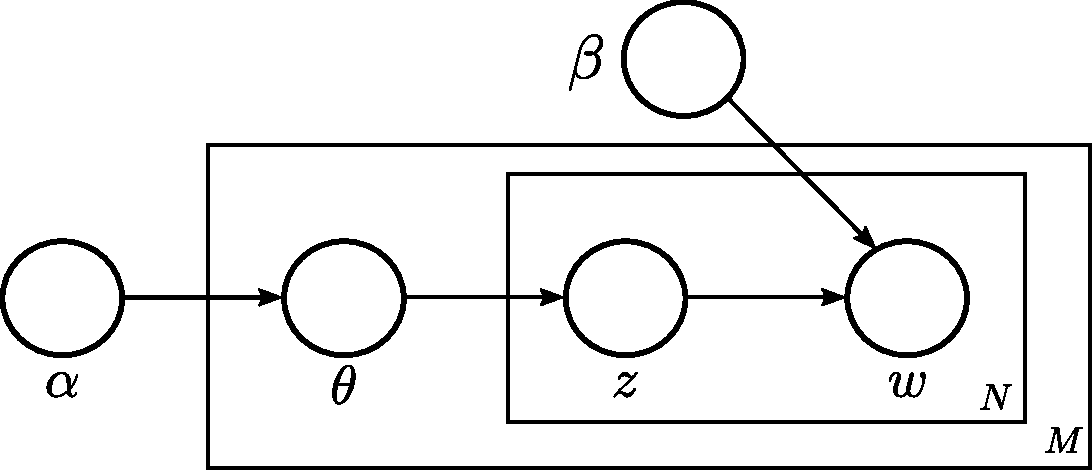
\includegraphics[width=0.5\textwidth]{./lda_plate.pdf}
\par\end{centering}
\caption{Graphical Model for LDA\label{fig:lda-graphical}}
\end{figure}

\subsection{Algorithm}
We present the basic variational expectation-maximization algorithm for estimating LDA parameters. A number of improvements on this have been presented, including Gibbs Sampling, Collapsed Gibbs Sampling, etc., which could potentially be incorporated down the road.

Assume we have been given a corpus of $M$ documents, call this $W$. Our goal is to learn values for parameters $\alpha$ and $\beta$ which maximize the log-likelihood of the observed corpus. The other unobserved variables, $Z$ and $\theta$, are treated as latent/nuisance variables. We can formulate this as:
\begin{align}
    \max_{\alpha, \beta} \log P(W | \alpha, \beta)
\end{align}
Because of the nuisance/latent variables $Z$ and $\theta$, this cannot be optimized directly. Instead, we derive a lower-bound on the log likelihood and maximize it:
\begin{align}
    \log P(W | \alpha, \beta)
    &= E_{Z, \theta \sim Q}\left[\log \frac{P(Z, \theta, W | \alpha, \beta)}{Q(Z, \theta)}\right] + D_{KL}(Q(Z, \theta) || P(Z, \theta | \alpha, \beta))\\
    &= \mathcal{L}(\alpha, \beta, Q) + D_{KL}(Q(Z, \theta) || P(Z, \theta | \alpha, \beta))
\end{align}
where $Q$ is an arbitrary variational distribution. Since the KL-divergence is non-negative, $\mathcal{L}(\alpha, \beta, Q)$ is a lower bound on the log-likelihood; thus it is often called a \textit{variational lower bound}. In some contexts it may also be referred to as the \textit{variational free energy}.

In EM, the variational lower bound $\mathcal{L}$ is maximized by co-ordinate ascent. In particular, in the E-step $\mathcal{L}$ is maximized with respect to the variational distribution over latent variables $Q$, while in the M-step $\mathcal{L}$ is maximized with respect to the parameters $\alpha$ and $\beta$.

\subsubsection{E-step}
To perform the E-step, we observe that $\log P(W | \alpha, \beta)$ does not depend on $Q$, so $\mathcal{L}$ is maximized with respect to $Q$ when the KL-divergence term is minimized, which is achieved when $Q(Z, \theta) = P(Z, \theta | W, \alpha, \beta)$. If $P(Z, \theta | W, \alpha, \beta)$ is tractable, then the E-step just consists of making this assignment. However, in many cases, including the one we are in, $P(Z, \theta | W, \alpha, \beta)$ will not tractable. Instead, we perform a variational approximation; we select a tractable, parameterized family of distributions, and then perform free-form optimization with respect to those parameters to obtain the parameter setting that minimizes the KL-divergence term.

We select a family of distributions in which the $\theta_i \independent z_{i, j} \forall j \in [N]$ and $z_{ij} \independent z_{i\ell} \forall j \neq \ell$. That is, within a given document, we are explicitly ignoring dependencies both between the topic distribution $\theta_i$ and topic variables $z_{ik}$, and between pairs of topic variables. The distribution takes the form:
\begin{align}
    Q(Z, \theta | \gamma, \phi) = \prod_{i=1}^M Q(Z_i, \theta_i) = \prod_{i=1}^M \left(Q(\theta_i | \gamma_i)\prod_{j=1}^N Q(z_{ij} | \phi_{ij})\right)
\end{align}
$\gamma_i \in \mathbb{R}^K_+$ is a set of variational parameters picking out a Dirichlet distribution for $\theta_i$. Likewise, $\phi_{ij} \in \Delta^{K-1}$ is a set of variational parameters picking out a Multinomial distribution for $z_{ij}$. The E-step then consists of solving the following optimization problem for the $i$-th document:
\begin{align}
    (\gamma^*_i, \phi^*_i) = \argmin_{\gamma_i, \phi_i} D_{KL}\left(Q(\cdot | \gamma_i, \phi_i) || P(\cdot | \alpha, \beta)\right)
\end{align}

\citet{blei2003latent} derive a co-ordinate descent algorithm for performing this optimization, whose updates take the form:
\begin{align}
    \phi_{ijk} &\propto \beta_{k, w_{ij}} \exp\{E_q[\log(\theta_{ik})]\} = \beta_{k, w_{ij}} \exp\{\Psi(\gamma_{ik}) - \Psi(\sum_{\ell = 1}^K \gamma_{i\ell})\}\\
    \gamma_{ik} &= \alpha_k + \sum_{j=1}^N \phi_{ijk}
\end{align}
where $\Psi(\cdot)$ is the Digamma function. Each update corresponds to completely (and in closed form) minimizing the KL-divergence w.r.t.\ one of the variables. For a given E-step, these updates are repeated until convergence.

\subsubsection{M-step}
Recall that the M-step consists of maximizing $\mathcal{L}(\alpha, \beta, Q)$ with respect to $\alpha$ and $\beta$. For $\beta$, the updates take the form:
\begin{align}
    \beta_{kw} \propto \sum_{i=1}^M \sum_{j=1}^N \phi_{ijk}\mathbbm{1}_{w_{ij} = w}
\end{align}
Basically, for each topic, the probability of each word is a normalized version of the sum of all the $\phi$ values for that topic-word combination. This comes from computing an M-projection of the distribution obtained by normalized the sum-of-phi's onto the space of multinomial distributions (i.e.\ the space of all discrete distributions; therefore no projection is really done at all). $L(\alpha, \beta, Q)$ is optimized w.r.t\ $\alpha$ using a fast Newton-Raphson method.

\begin{codebox}
\Procname{$\proc{E-Step}(W, \beta, \alpha)$}
\li\For$i \gets 1$ \To$M$
\li    \Do$\gamma^0_{ik} = \alpha_k+ N/K$ for all $j \in[K]$
\li    $\phi^0_{ijk} = 1/K$ for all $j \in[N], k \in[K]$
\li    $t \gets 0$
\li    \While\text{not converged}
\li        \Do\For$j \gets 1$ \To$N$
\li            \Do\For$k \gets 1$ \To$K$
\li                \Do$\phi^{(t+1)}_{ijk} \gets \beta_{k,w_{ij}} \exp\{\Psi(\gamma^{(t)}_{ik})\}$
                \End
\li            Normalize $\phi_{ij\cdot}$ to sum to 1
            \End
\li        \For$k \gets 1$ \To$K$
\li            \Do$\gamma^{(t+1)}_{ik} \gets \alpha_k+ \sum_{j=1}^N \phi^{(t+1)}_{jk}$
            \End
\li        $t \gets t + 1$
        \End
    \End
\li\Return$(\gamma, \phi)$
\end{codebox}

\begin{codebox}
\Procname{$\proc{M-Step}(W, \beta, \alpha)$}
\li\For$k \gets1$ \To$K$
\li     \Do \For $w \gets 1$ \To$M$
\li         \Do \For
        \End
    \End
\li\Return$(\gamma, \phi)$
\end{codebox}

\begin{codebox}
\Procname{$\proc{Latent-Dirichlet-Allocation}(W, \beta, \alpha)$}
\li$t \gets0$
\li\While\text{not converged}
\li    \Do$(\gamma, \phi) \gets \proc{E-Step}(W, \beta, \alpha)$
\li    $(\beta, \alpha) \gets \proc{M-Step}(W, \gamma, \phi)$
\li    $t \gets t + 1$
   \End
\end{codebox}

\section{Modelling Topics as Sequence Generators}
In the vanilla LDA model just described, the topic-conditional distributions over words (i.e.\ the rows of $\beta$) are allowed to be any discrete distribution. For applications where there are a large number of possible words (i.e.\ if the words are long sequences of characters), the number of parameters to learn can grow to be unmanageable, and can make it difficult to obtain enough data to avoid over-fitting. We can remedy this by considering constrained families of distributions over strings with significantly fewer parameters to learn, reulting in a tangible decrease in sample complexity in applications where such constraints are deemed appropriate. We first consider using Markov Chains as the topic-conditional distributions, and move on to consider two generalizations thereof, namely hidden markov models and probabilistic finite automata. Making this change also provides a tidy solution to the problem of dealing with words that occur in the test set but not the training set. Markov Chains and Hidden Markov Models readily provide reasonable estimates of the probability of such words, while unconstrained multinomials have a more difficult time.

\subsection{Markov Chain Topics}
Modelling topic-conditional distributions using sequence models requires new notation. Let $\Sigma = [S]$ be our alphabet, where $S \in \mathbb{N}$ is the number of symbols. Denote the set of finite-length strings by $\Sigma^* = \bigcup_{k=0}^\infty \Sigma^k$. There are many ways of viewing Markov Chains, but for our purposes we will say that a Markov Chain is a tuple $\langle \pi, T\rangle$ where $\pi \in \mathbb{R}^{|\Sigma|}$ is a vector such that $\pi(i)$ gives the probability that the first symbol is $i$, $T \in \mathbb{R}^{|\Sigma| \times |\Sigma|}$ is a matrix such that $T_{i,j} = T(j | i)$ gives the probability of emitting symbol $j$ given we have just emitted symbol $i$ and $h \in \mathbb{R}^{|\Sigma|}$ is a vector such that $h(i)$ gives the probabilty of halting given that we have just emitted symbol $i$. Also, all parameters are between 0 and 1, and $\sum_{j=1}^{|\Sigma|} T(j | i) + h(i) = 1$. A Markov Chain defines a distribution over strings of arbitrary length (elements of $\Sigma^*$) with a probability mass function given by $P(x) = \pi(x_1) \prod_{i=1}^{n-1} T(x_{j+1} | x_j) h(x_n)$, assuming $x = x_1x_2 \dots x_n \in \Sigma^*$. Alternatively, a Markov Chain can be seen to specify a distribution over strings of a fixed length $L$ (elements of $\Sigma^L$) by setting $h(i) = 0~\forall i$, and taking $P(x) = \pi(x_1) \prod_{i=1}^{L-1} T(x_{j+1} | x_j)$, corresponding to artificially halting the generation process after $L$ symbols, though we will not make use of this formulation in the current work.

\begin{figure}[h!]
\begin{centering}
    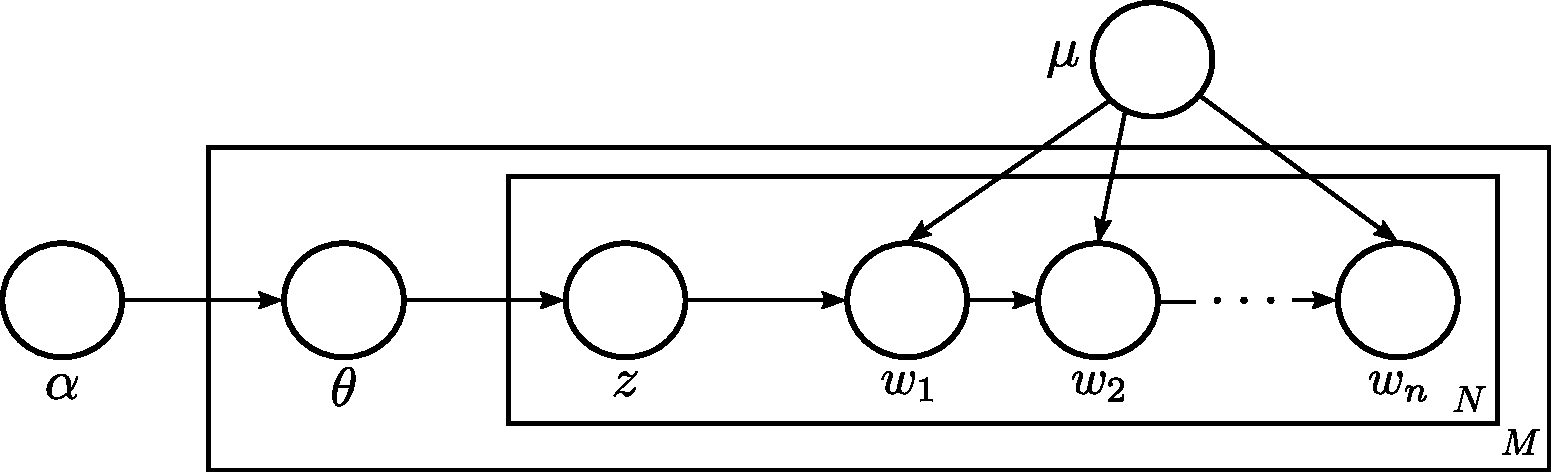
\includegraphics[width=\textwidth]{./lda_mm_plate.pdf}
\par\end{centering}
\caption{Graphical Model for LDA with Markov Chain Topics\label{fig:lda-graphical-markov}}
\end{figure}

A Markov Chain is a relatively compact way of specifying a distribution over strings of arbitrary length, requiring just $(|\Sigma| + 1)(|\Sigma| - 1)$ parameters (since each of the $|\Sigma| + 1$ multinomial distributions that make up a Markov Chain requires $|\Sigma| - 1$ parameters). The price paid for this representational efficiency is of course reduced expressivity; the space of string distributions that can be described via a Markov Chain is a small subset of the space of all possible string distributions.

\subsection{Algorithm}
Altering LDA to use Markov Chain topics is a relatively simple matter. Let $\mu^{(k)} =  \langle \pi^{(k)}, T^{(k)}, h^{(k)} \rangle$ be the Markov Chain for the $k$-th topic for $k \in [K]$, and let $\mu = \{\mu^{(1)}, \mu^{(2)}, \dots, \mu^{(k)}\}$ stand in for the collection all the parameters for all topics (so $\mu$ replaces $\beta$ from standard LDA). In the E-step, nothing changes except that rather than storing $\beta_{kw}$ in a matrix, we compute $\beta_{kw} = P(w) = \pi(w_1) \prod_{i=1}^{n-1} T(w_{i+1}| w_i) h(w_n)$. The M-step consists of learning parameters for the Markov Chains. We want to solve:
\begin{align}
    \mu^*
    &= \argmax_{\mu} L(\alpha, \mu, Q)\\
    &= \argmax_{\mu} E_{Z, \theta \sim Q}\left[\log \frac{P(Z, \theta, W | \alpha, \mu)}{Q(Z, \theta)}\right]\\
    &= \argmax_{\mu} \sum_{Z, \theta}Q(Z, \theta) \log \frac{P(Z, \theta, W | \alpha, \mu)}{Q(Z, \theta)}\\
    &= \argmax_{\mu} \sum_{Z, \theta}Q(Z, \theta) \log P(Z, \theta, W | \alpha, \mu)~\text{(removing a term which does not depend on $\mu$)}\\
    &= \argmax_{\mu} \sum_{Z, \theta}Q(Z, \theta) \log P(W | Z, \mu) P(Z | \theta) P(\theta | \alpha)~\text{(applying factorization of $P(Z, \theta, W | \alpha, \mu)$ given by the Bayes net)}\\
    &= \argmax_{\mu} \sum_{Z, \theta}Q(Z, \theta) \log P(W | Z, \mu)~\text{(removing term which do not depend on $\mu$)}\\
    &= \argmax_{\mu} \sum_{Z}Q(Z) \log P(W | Z, \mu)~\text{(marginalizing out $\theta$)}\\
    &= \argmax_{\mu} \sum_{i=1}^M \sum_{j=1}^N \sum_{k=1}^K Q^k_{ij}(z_{ij}) \log P(x_{ij} | z_{ij} = k, \mu)~\text{(using the fact that $P(W | Z, \mu)$ factors completely)}\\
    &= \argmax_{\mu} \sum_{k=1}^K \left(\sum_{i=1}^M \sum_{j=1}^N \phi_{ijk}\right) \log P(x_{ij} | z_{ij} = k, \mu^{(k)})
\end{align}
Now considering each $\mu^{(k)}$ separately, we have to optimize:
\begin{align}
    &= \argmax_{\mu^{(k)}} \left(\sum_{i=1}^M \sum_{j=1}^N \phi_{ijk}\right) \log P(x_{ij} | z_{ij} = k, \mu^{(k)})\\
    &= \argmax_{\mu^{(k)}} \sum_{w=1}^W \left(\sum_{i=1}^M \sum_{j=1}^N \phi_{ijk} \mathbbm{1}_{x_{ij} = w}\right) \log P(x = w | z = k, \mu^{(k)})
\end{align}
This is equivalent to maximizing (minimizing) a negative (positive) cross-entropy between a distribution defined by $P_k(x = w) \propto \sum_{i=1}^M \sum_{j=1}^N \phi_{ijk}\mathbbm{1}_{x_{ij} = w}$ and the distribution defined by the $k$-th Markov Chain. Moving on:
\begin{align}
    &= \argmax_{\mu^{(k)}} \sum_{w=1}^W P_k(x = w) \left(\log \pi^{(k)}(w_1) + \sum_{a, b \in \Sigma} n_{a, b}^w \log T^{(k)}(b | a) + \log h^{(k)}(w_n)\right)
\end{align}
This yields a number of separable optimization problems. Considering first the optimization in $\pi^{(k)}$:
\begin{align}
    &= \argmax_{\pi^{(k)}} \sum_{w=1}^W P_k(x = w) \log \pi^{(k)}(w_1)\\
    &= \argmax_{\pi^{(k)}} \sum_{\sigma \in \Sigma} \sum_{w=1}^W P_k(x = w)\mathbbm{1}_{w_1 = \sigma} \log \pi^{(k)}(\sigma)
\end{align}
Here we are maximizing a discrete negative cross-entropy between an unnormalized distribution and $\pi^{(k)}(\cdot)$. The solution thus has the form:
\begin{align}
    \pi^{(k)}(\sigma) \propto \sum_{w=1}^W P_k(x = w)\mathbbm{1}_{w_1 = \sigma} 
\end{align}
For optimizing w.r.t.\ $T^{(k)}$ and $h^{(k)}$, we consider each symbol separately. For $\sigma \in \Sigma$:
\begin{align}
    &= \argmax_{T^{(k)}(\cdot | \sigma), h^{(k)}(\sigma)} \sum_{w=1}^W P_k(x = w) \left(\sum_{\ell} n_{\sigma,\ell}^w \log T^{(k)}_{\sigma, \ell} + \mathbbm{1}_{w_{-1}=\sigma}\log h^{(k)}(\sigma)\right)\\
    &= \argmax_{T^{(k)}(\cdot | \sigma), h^{(k)}(\sigma)} \sum_{\ell \in \Sigma} \left( \sum_{w=1}^W P_k(x = w)n^w_{\sigma,\ell}\right)\log T^{(k)}_{\sigma, \ell} + \left( \sum_{w=1}^W P_k(x = w)\mathbbm{1}_{w_{-1}=\sigma}\right)\log h^{(k)}(\sigma)
\end{align}
If we take $T^{(k)}(\cdot | \sigma)$ and $h^{(k)}(\sigma)$ as together defining a distribution over what happens after the symbol $\sigma$ is emitted, then we can use the same cross-entropy argument as before to conclude:
\begin{align}
    T^{(k)}_{\sigma, \ell} \propto \sum_{w=1}^W P_k(x = w)n_{\sigma,\ell}^w && h^{(k)}(\sigma) \propto \sum_{w=1}^W P_k(x = w)\mathbbm{1}_{w_{-1}=\sigma}
\end{align}

\subsection{Time Complexity}
\subsubsection{E-Step}
All that changes on the E-step is how $\beta_{k,w}$ is computed. A naive implementation that computes $\beta$ by brute force would require an extra step for each E-step, the time complexity of which would be $O(K V \overline{|w|})$ where $\overline{|w|}$ is the average length  of words in the training set. However, it is likely that by storing the training words in a structure such as a suffix tree, the dependence on word-length can be significantly reduced. The algorithm would be something like: at the beginning of training, build a suffix tree from the training data. Then on each E-step, for each topic, create an annotated suffix tree where each edge is annotated by the probability that edge receives from the Markov Chain for that topic. Then traverse the suffix tree in order to fill in $\beta_k$. Should give a speedup, especially for datasets with small alphabets.

The complexity of the $E$-step in vanilla LDA is $O(MNKf(W))$, where $f(W)$ is the average number of iterations required for the variational optimization to converge. \citep{blei2003latent} found empirically that $f(W)$ tends to be on the order of $N$ (the number of words per document), yielding an approximate complexity of $O(MN^2K)$ per $E$-step.

\subsubsection{M-Step}
We'll consider only maximizing $\mathcal{L}(\alpha, \mu, Q)$ w.r.t.\ $\mu$, since the maximization w.r.t.\ $\alpha$ is the same for our modified algorithm as it is for vanilla LDA. In vanilla LDA, solving for $\beta$ during the $M$-step requires $O(VK)$ runtime, since computing the sufficient statistics of $\phi$ and $\gamma$ which are necessary for the optimization can be folded into the E-step without changing its complexity. For our algorithm, the complexity of the $M$-step is $O(VK\overline{|W|_{trans}})$ where $\overline{|W|_{trans}}$ is the average number of unique transition types per word (e.g.\ if $\Sigma = \{0, 1\}$, then there are 4 possible transition types, but many words will have fewer than that. For example, $00000011111$ has only 3 transition types). The number of transition types in a word is always less than the length of the word, possibily signficantly so if the words are long and the alphabet is small.

\begin{figure}[h!]
\begin{centering}
    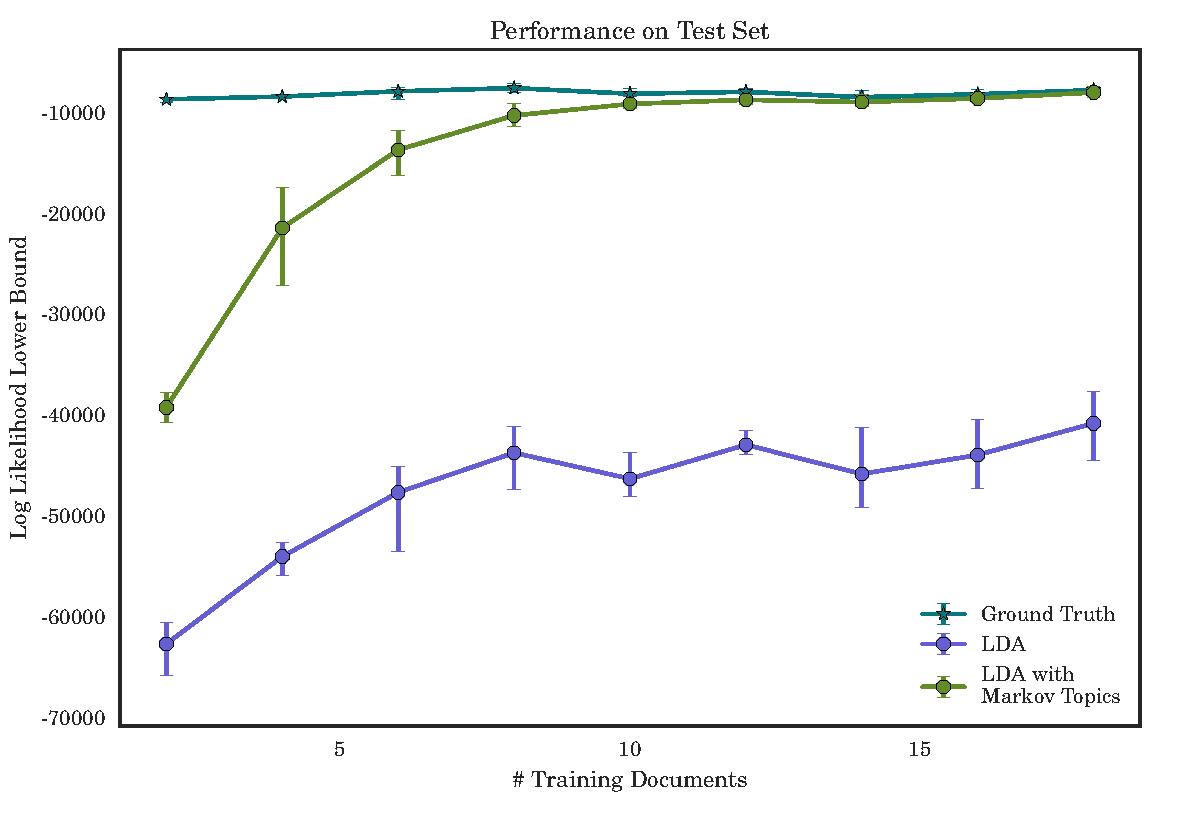
\includegraphics[width=1.0\textwidth]{./markov_model_medium_likelihood_vs_n_train}
\par\end{centering}
\caption{3 topic, 10 characters, 100 words per doc \label{fig:results}}
\end{figure}
\begin{figure}[h!]
\begin{centering}
    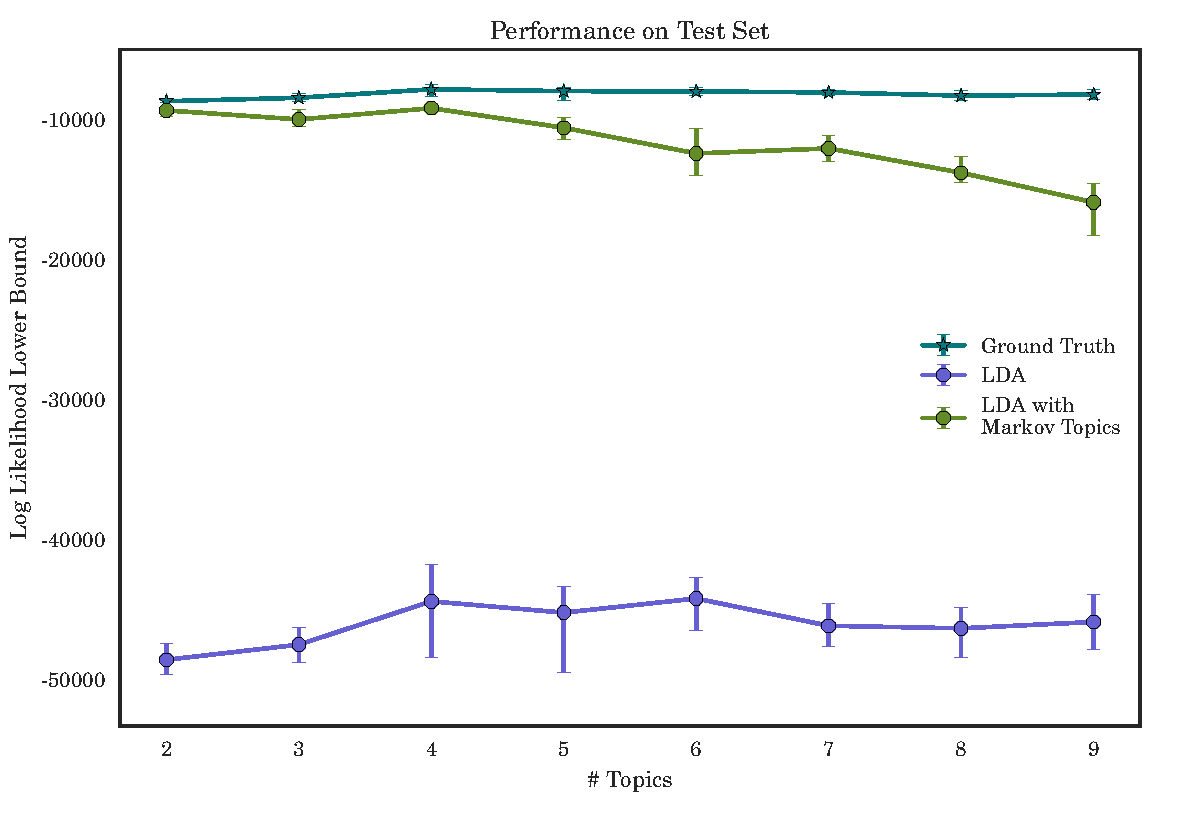
\includegraphics[width=1.0\textwidth]{./markov_model_medium_likelihood_vs_n_topics}
\par\end{centering}
\caption{10 training docs, 10 characters, 100 words per doc \label{fig:results1}}
\end{figure}


\bibliographystyle{apalike}
\bibliography{/home/eric/Dropbox/library}

\end{document}
